\chapter{802.11ax Features}			\label{chp_ax_feature}
The legacy random access is called distributed coordination function (DCF). 
Since the DCF degrades performance severely at dense scenario solution, IEEE 802.11ax proposes a centralized coordination MAC, improving the status of AP. 
This centralized coordination function is also based on DCF so that 802.11ax is compatible with legacy 802.11 and other wireless system. 
At the same time, multi-user (MU) PHY is issued in IEEE 802.11ax to improve the system performance\cite{dengquality}. 
In this chapter, we first introduce 802.11ax feature, MU PHY, then illustrate the OFDMA-based random access mechanism.
\section{Multi-User PHY} \label{sec_MU}
\subsection{PHY}
While legacy 802.11 specifies a 20 MHz channel a Single User (SU) channel, which means only one user could access the channel at a time in a BSS, 802.11ax issues a MU PHY with OFDMA, allowing multiple STAs to access channel simultaneously.
It should help mitigate contention and collision. 

The channel in 802.11ax is more fine-grained, defined as resource unit (RU) in figure \ref{fig_RU_spec}. 
The smallest RU is 26-tone, with which a legacy 20 MHz channel could be separated into 9 subchannels.
It is flexible that if there are not 9 HE-STAs to share the channel, AP could allocate multiple RUs to one HE-STA without wasting the RUs.
And as specified in figure \ref{fig_RU_spec}, multiple 20 MHz channels can be aggregated to be utilized by a BSS, which is called \textit{Channel Bonding}. 
This will help a lot improve system performance, since one BSS is not restricted to a single 20 MHz channel.  
It is worth mentioning that every transmission of MU should end at the same time. That means padding is required for short packets.



Actually, DL MU PHY has been implemented in 802.11n and 802.11ac with MU-MIMO, which is an absolutely different method from OFDMA and beyond the scope of this paper. 

\begin{figure}[!t]
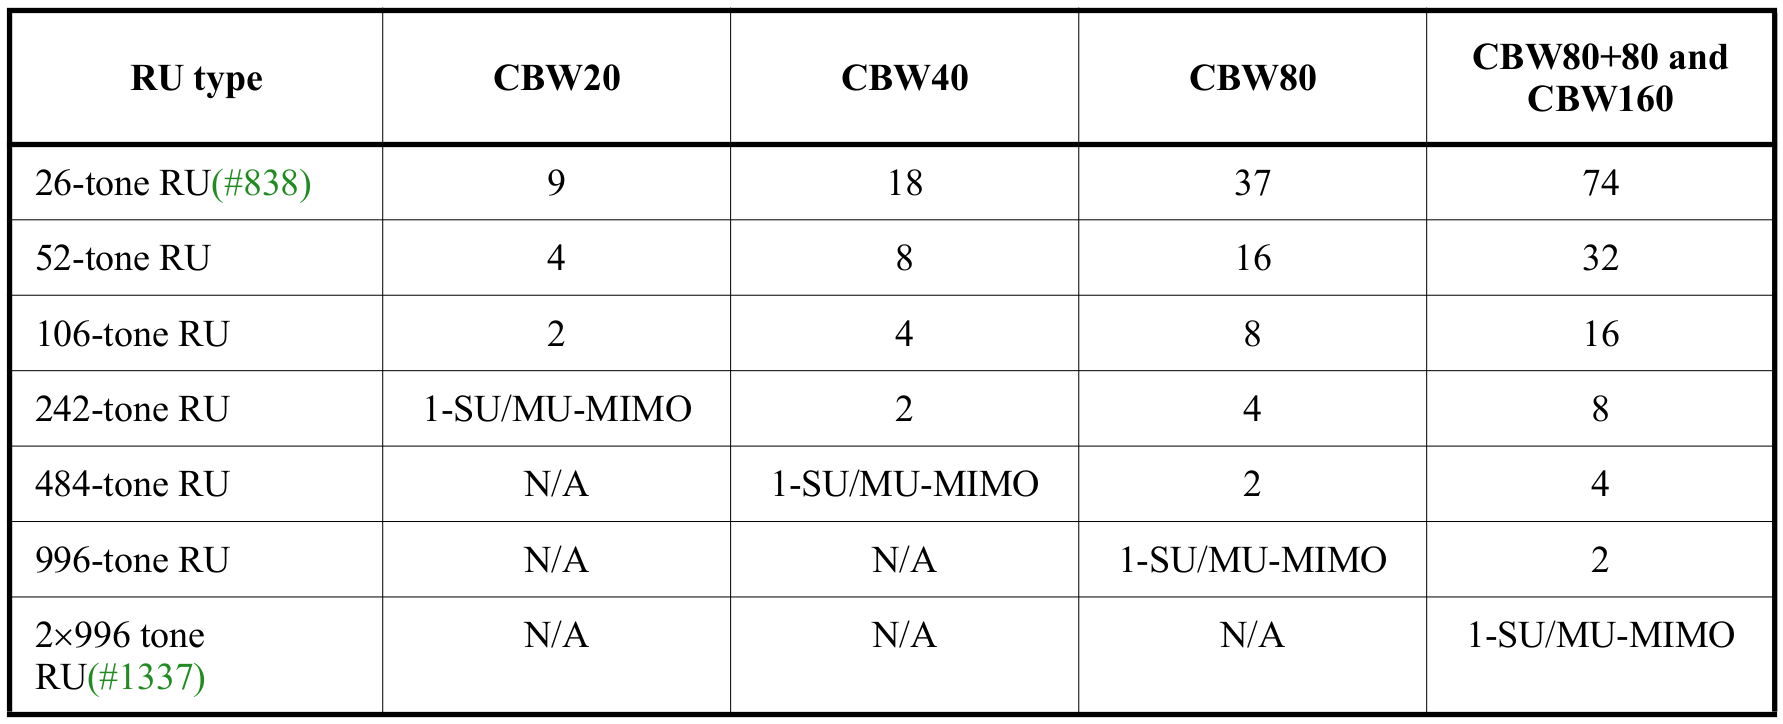
\includegraphics[scale=0.25]{./figure/chp2/RU_spec.png}
\caption{Maximum number of RUs for each channel width}
\label{fig_RU_spec}
\end{figure}


\begin{figure}[!t]
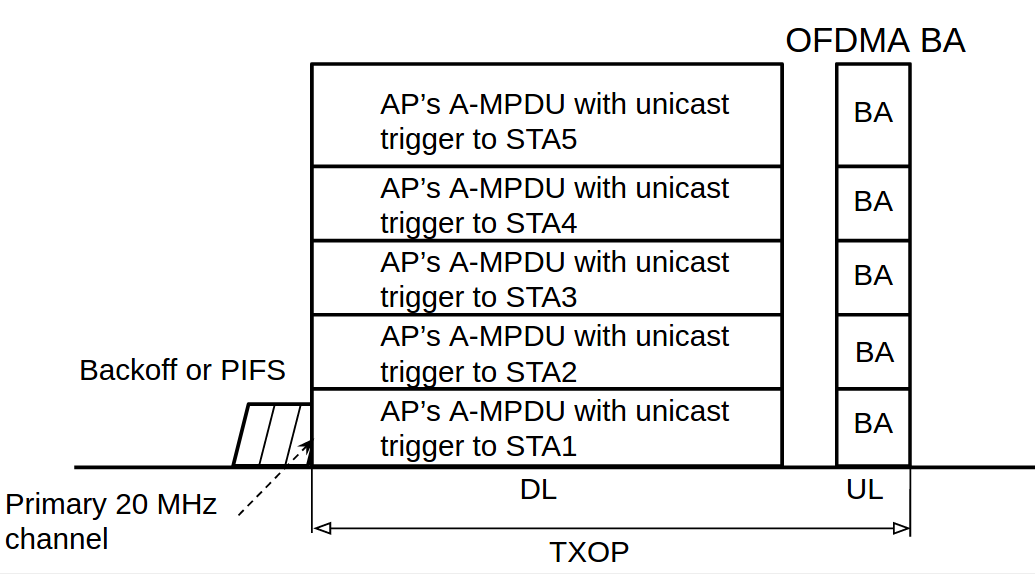
\includegraphics[scale=0.4]{./figure/chp2/fig_MU_DL.png}
\caption{MU DL of 802.11ax}
\label{fig_MU_DL}
\end{figure}


\begin{figure}[!t]
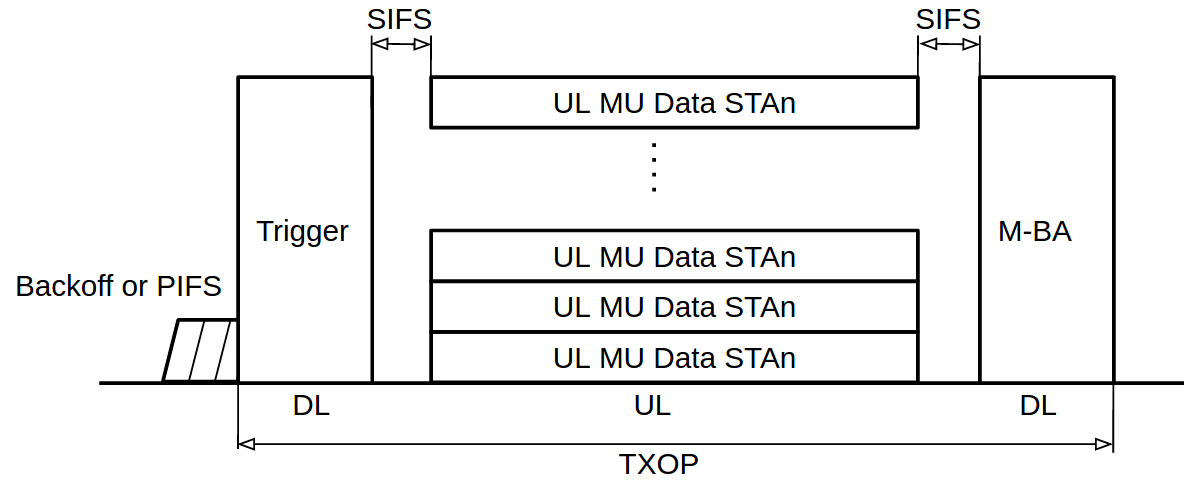
\includegraphics[scale=0.36]{./figure/chp2/fig_MU_UL.png}
\caption{Trigger-based MU UL of 802.11ax}
\label{fig_MU_UL}
\end{figure}


\subsection{MAC}
802.11ax MAC is still based on DCF. However, only AP follows DCF. HE-STAs are scheduled by AP.
AP will contend with DCF procedure to transmit DL packets with OFDMA to multiple stations, which is called MU DL as in figure \ref{fig_MU_DL}. 
The difficulty of OFDMA MU is MU UL. 
802.11 is not a synchronous system, preamble and even two-way handshaking are required before a data transmission. 
A trigger-based MU UL is issued as in figure \ref{fig_MU_UL}.
A brand new control frame, called trigger frame, is created to be transmitted by AP before HE-STAs transmitting a UL packet. 
In this way, stations are able to access channel with RU scheduled by trigger frame transmitted by AP. 
The trigger frame format is as figure \ref{fig_TF_format}. Since the standard is in progress, many fields remain to be determined (TBD). 

\begin{figure}[!ht]
\centering
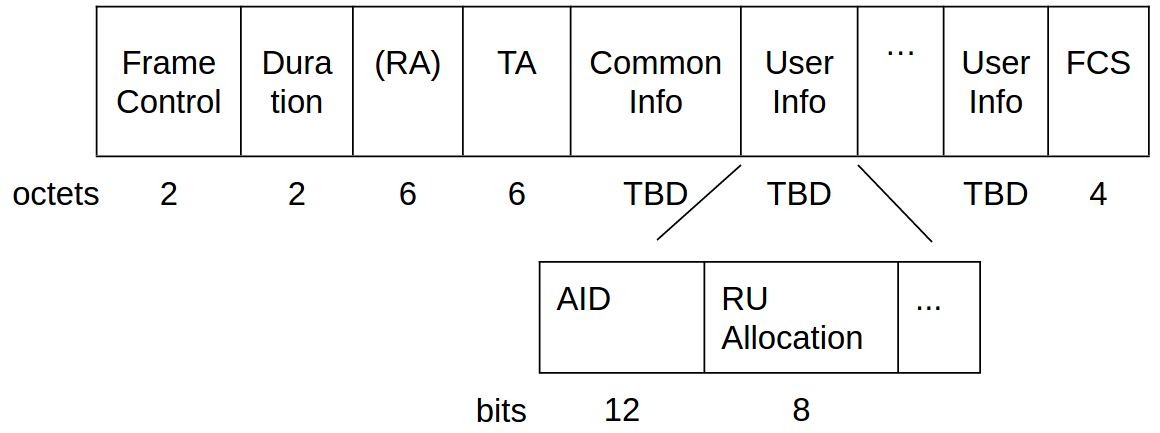
\includegraphics[scale=0.3]{./figure/chp2/fig_tf_format.png}
\caption{Trigger Frame format}
\label{fig_TF_format}
\end{figure}

The basic use of trigger frame is to allocate RUs. It contains resource allocation information in field \textit{user info}, specifying some station to access some RU in subfield \textit{AID} and \textit{RU allocation}.  
When AP schedules RUs for random access, the subfield \textit{AID} of User Info is set to value 0. The detailed procedure we will illustrate in section \ref{sec_RA_illu}. 

What's more, to support scheduling of TF, a mechanism called \textit{Target Wake Time} (TWT) is implemented in 802.11ax. TWT is originally issued in 802.11ah for power saving\cite{khorov2015survey}. It is also out of scope of this thesis.



\section{802.11ax Random Access Illustration}		\label{sec_RA_illu}
\begin{figure*}[!t]
%\begin{minipage}{.5\textwidth}
\centering
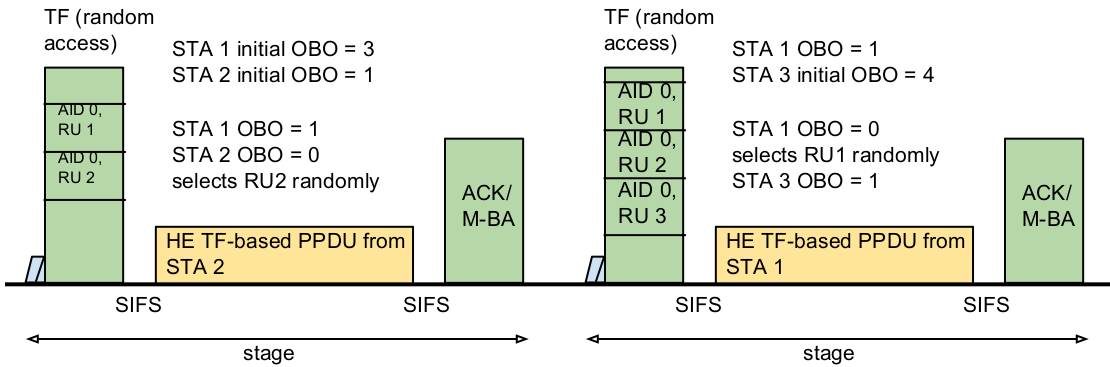
\includegraphics[scale=0.35]{./figure/chp2/RA_illu.png}
\caption{Illustration of OFDMA-based random access}
\label{fig_ra_illu}
%\end{minipage}
\end{figure*}

%\begin{minipage}{.5\textwidth}
%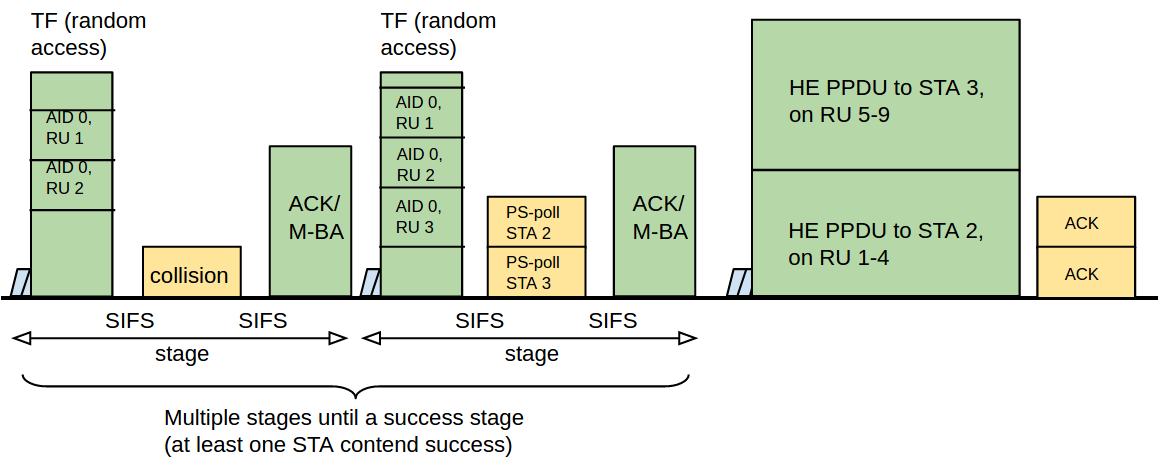
\includegraphics[scale=0.35]{./figure/RA_illu_3.png}
%\caption{Another example of OFDMA-based random access for DL in 802.11ax}
%\label{fig_ra_dl}
%\end{minipage}


\begin{figure}[!t]
\centering
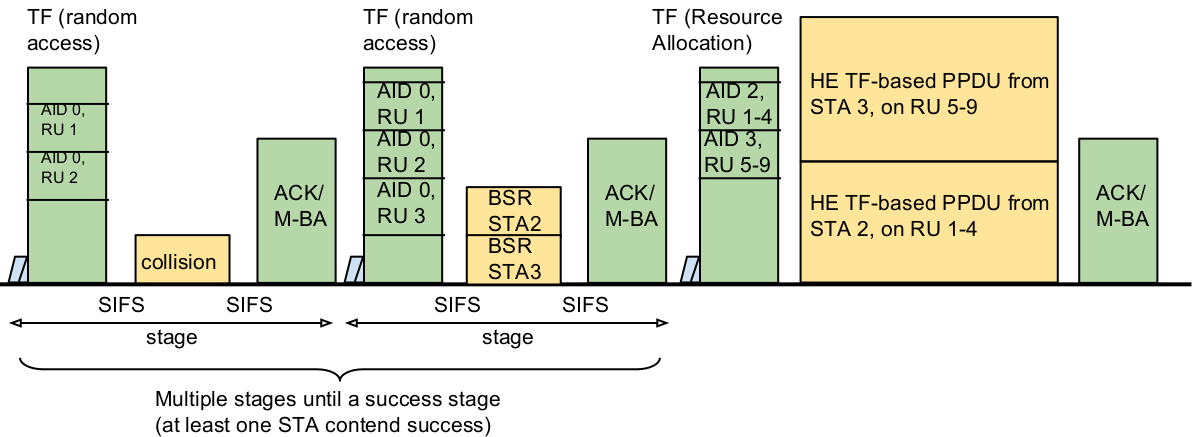
\includegraphics[scale=0.35]{./figure/chp2/RA_illu_2.png}
\caption{An example of OFDMA-based random access for UL in 802.11ax}
\label{fig_ra_ul}
\end{figure}

As stated above, legacy IEEE 802.11 MAC is a 20 MHz SU PHY, which means that at most single user could succeed in contending at a time slot.
With the MU PHY, HE-STA (802.11ax, high efficient station) has multiple RUs to access, which means multiple HE-STAs may access channel at the same time.
And the system parameters are set by AP dynamically.
The procedure is of course more complicated and flexible.
We first illustrate the OFDMA-based random access procedure then give one use case of the random access.

Different from legacy 802.11 where parameters like contention window are pre-set at hardware of station, all the parameters are configured by AP in 802.11ax. 
The parameter set is composed of $OCW_{min}, OCW_{max}, M$. $OCW_{min}$, (i.e., OFDMA contention window), represents the minimum contention window, while $OCW_{max}$ represents the maximum contention window. 
And $M$ is the number of RUs for random access. $OCW_{min}, OCW_{max}$ are given in an element called RAPS (random access parameter set) contained in beacon frame sent by AP.
In this way, HE-STA is able to access channel with different parameters obtained from the beacon frame. 


In a beacon interval, to initialize a random access procedure, AP first transmits a trigger frame. 
The TF announces some RUs for random access by setting the AID of those RUs value of 0. 
HE-STAs need to maintain a backoff counter, called OFDMA Backoff (OBO). 
HE-STAs who want to access channel will randomly generate a OBO among range $[0, OCW_i]$, where $i$ is the backoff level and $OCW$ is retrieved from RAPS sent by AP. 
Then the OBO subtracts $M$, the value of number of RUs for random access in the current stage. 
If the OBO reaches 0, the HE-STA will randomly select a RU from those RUs for random access to transmit a packet after SIFS (short inter-frame spacing). 
After that AP responds with a block ACK indicating who succeed in contending.
The OFDMA-based random access is a three-way handshake, which is totally called a stage. 
It is worth reminding that the stage in this thesis is a concept of interval\cite{draft_ax}, not the backoff stage in papers\cite{bianchi2000performance}. 
To distinguish the two words, we use backoff level replacing backoff stage. 
Those whose OBO is greater than 0 will freeze the OBO and wait for next stage.  
If more than one HE-STA transmit at the same RU, collision occurs. 
Those who collide in the current stage will double their $OCW$ at next stage until $OCW$ reaches $OCW_{max}$. 
Only if at least one HE-STA succeed in transmit a request in a stage will the stage be a successful stage. 

Figure \ref{fig_ra_illu} illustrates the procedure. Green means transmission from AP to STA (i.e., DL) and yellow means UL direction. 
With clear illustration above, we look deeply into the implementation of the mechanism.
See figure \ref{fig_RAPS}, the two critical parameters $OCW_{min},OCW_{max}$ are specified in field OCW Range. 
The value is defined by $OCW_{min} = 2^{EOCW_{min}}-1$, $OCW_{max} = 2^{EOCW_{max}}-1$. 
In the following analysis, we issue another parameter $m$ so that maximum backoff level, $OCW_{max} = (OCW_{min}+1)*2^m-1$. So we specify $OCW_{max}$ with $m$ and $OCW_{min}$ in following section, which simplifies analysis.


Following is a use case of OFDMA-based random access as figure \ref{fig_ra_ul}. 
When HE-STAs want to random access to transmit data packets, he will send buffer state report (BSR) frame with OFDMA-based random access. 
After successful contention, AP will allocate RUs for the HE-STA by trigger frame.
Then stations transmit UL data packets with the allocated RUs. 


Other use cases could borrow the same random access procedure. 
Similar to legacy 802.11 power save, HE-STA needs to transmit PS-poll or APSD-trigger frame to inform AP of its active state when the HE-STA wakes up.
The transmission of PS-poll or APSD-trigger frame is a good case of OFDMA-based random access. After successful contention, AP will transmit the buffered packets of the HE-STA.

\begin{figure}[!h]
\centering
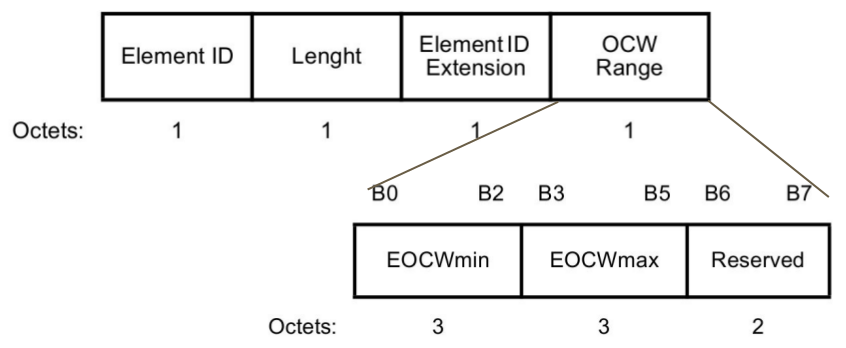
\includegraphics[scale=0.4]{./figure/chp2/RAPS.png}
\caption{Random Access Parameter Set (RAPS) Element}
\label{fig_RAPS}
\end{figure}

